% This document is compiled using XeLaTeX
\documentclass{article}

% 中文支持
\usepackage{xeCJK} % 支持中文
\setmainfont{Times New Roman} % 设置英文字体

% 其他常用包
\usepackage{graphicx} % 插入图片
\usepackage{enumerate} % 自定义列表

% 文档信息
\title{数字逻辑实验报告}
\author{雷业成 241220106}
\date{\today}

\begin{document}

\maketitle

\section{实验目的}
\begin{enumerate}
  \item 熟悉 Logisim 软件的使用方法;
  \item 掌握使用晶体管实现基本逻辑部件的方法;
  \item 利用基础元器件库设计简单数字电路;
  \item 了解子电路的设计和应用;
  \item 掌握分线器、隧道、探针等 Logisim 组件的使用方法。
\end{enumerate}

\section{实验环境}
Logisim:https://github.com/Logisim-Ita/Logisim

\section{实验内容}
\subsection{利用基本逻辑门设计一个3输入多数表决器}
\subsubsection{整体方案设计}
\begin{enumerate}
    \item 顶层方案设计
    \item 输入输出引脚
\end{enumerate}

\subsubsection{原理图和电路图}
\begin{figure}[htb]
  \centering
  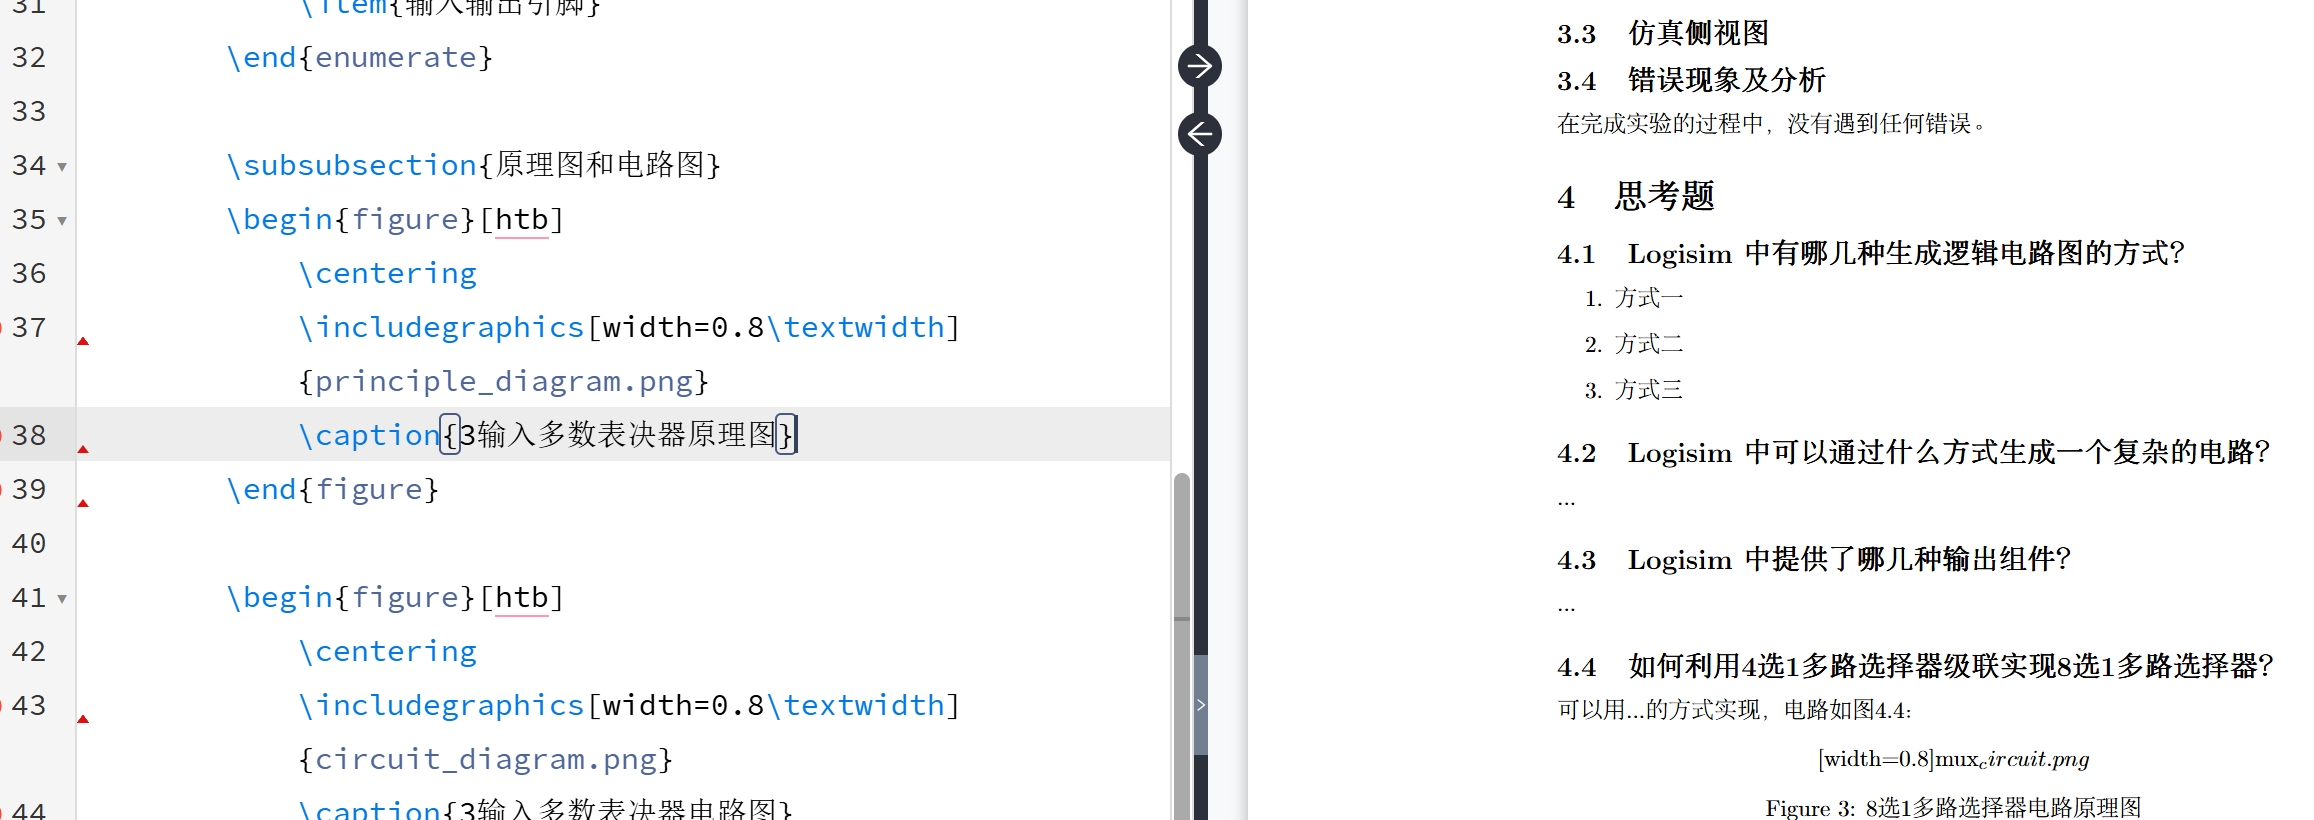
\includegraphics[width=0.8\textwidth]{image.png} % 替换为实际图片文件
  \caption{3输入多数表决器原理图}
\end{figure}

\begin{figure}[htb]
  \centering
  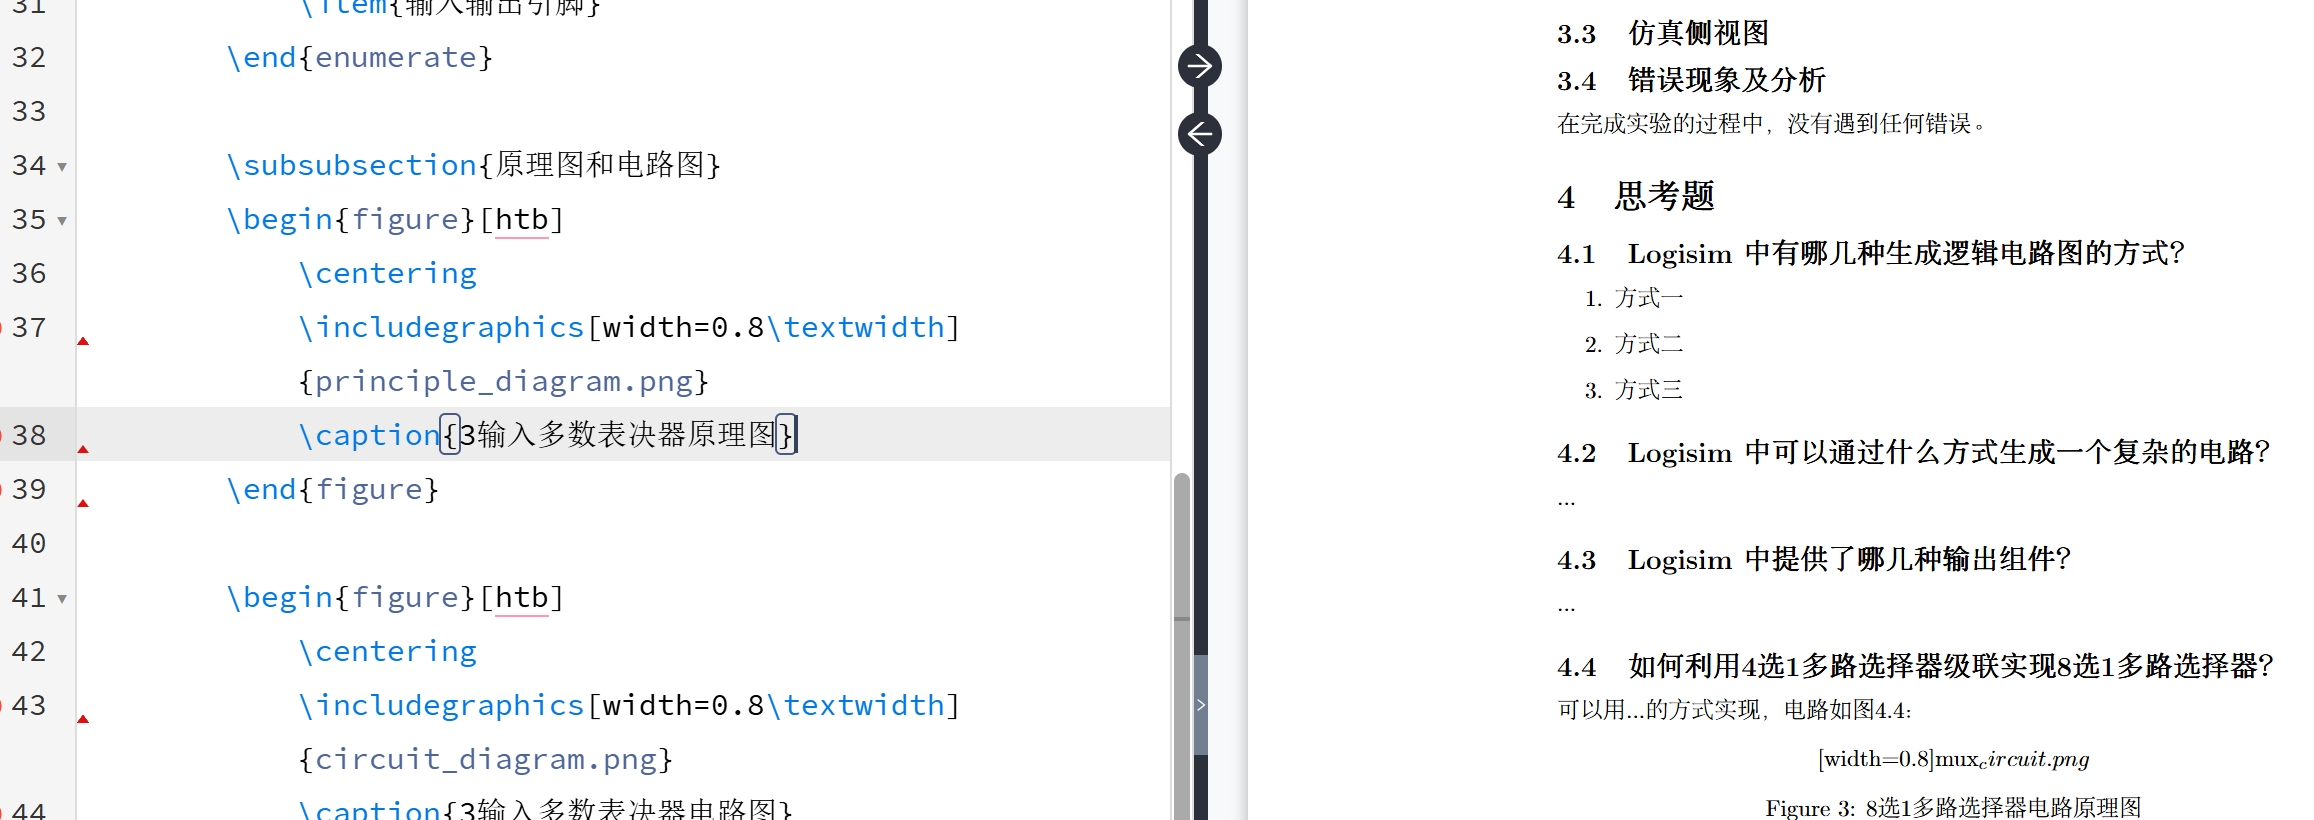
\includegraphics[width=0.8\textwidth]{image.png} % 替换为实际图片文件
  \caption{3输入多数表决器电路图}
\end{figure}

\subsection{实验步骤}
(此处填写实验步骤)

\subsection{仿真侧视图}
\begin{figure}[htb]
  \centering
  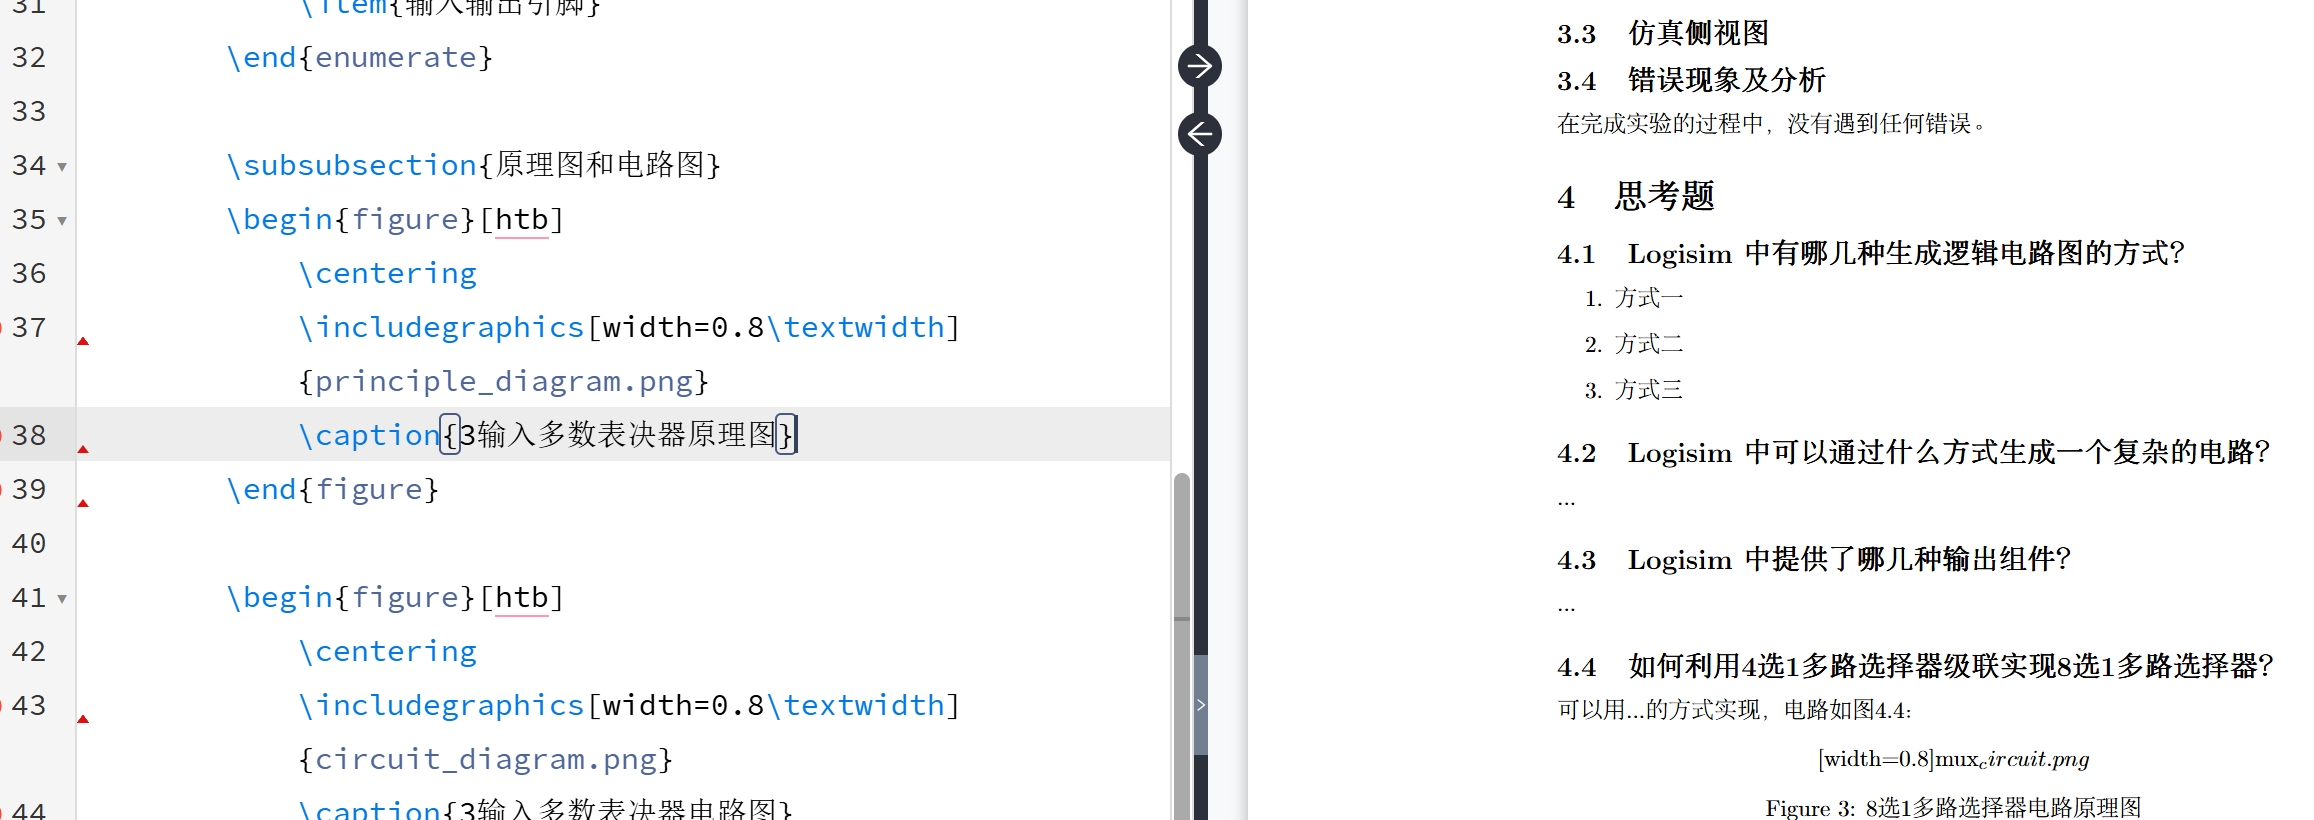
\includegraphics[width=0.8\textwidth]{image.png} % 替换为实际图片文件
  \caption{仿真侧视图}
\end{figure}

\subsection{错误现象及分析}
在完成实验的过程中,没有遇到任何错误。

\section{思考题}
\subsection{Logisim 中有哪几种生成逻辑电路图的方式?}
\begin{enumerate}
  \item 方式一
  \item 方式二
  \item 方式三
\end{enumerate}

\subsection{Logisim 中可以通过什么方式生成一个复杂的电路?}
(此处填写答案)

\subsection{Logisim 中提供了哪几种输出组件?}
(此处填写答案)

\subsection{如何利用4选1多路选择器级联实现8选1多路选择器?}
可以用级联的方式实现,电路如图\ref{8-1MUX}:

\begin{figure}[htb]
  \centering
  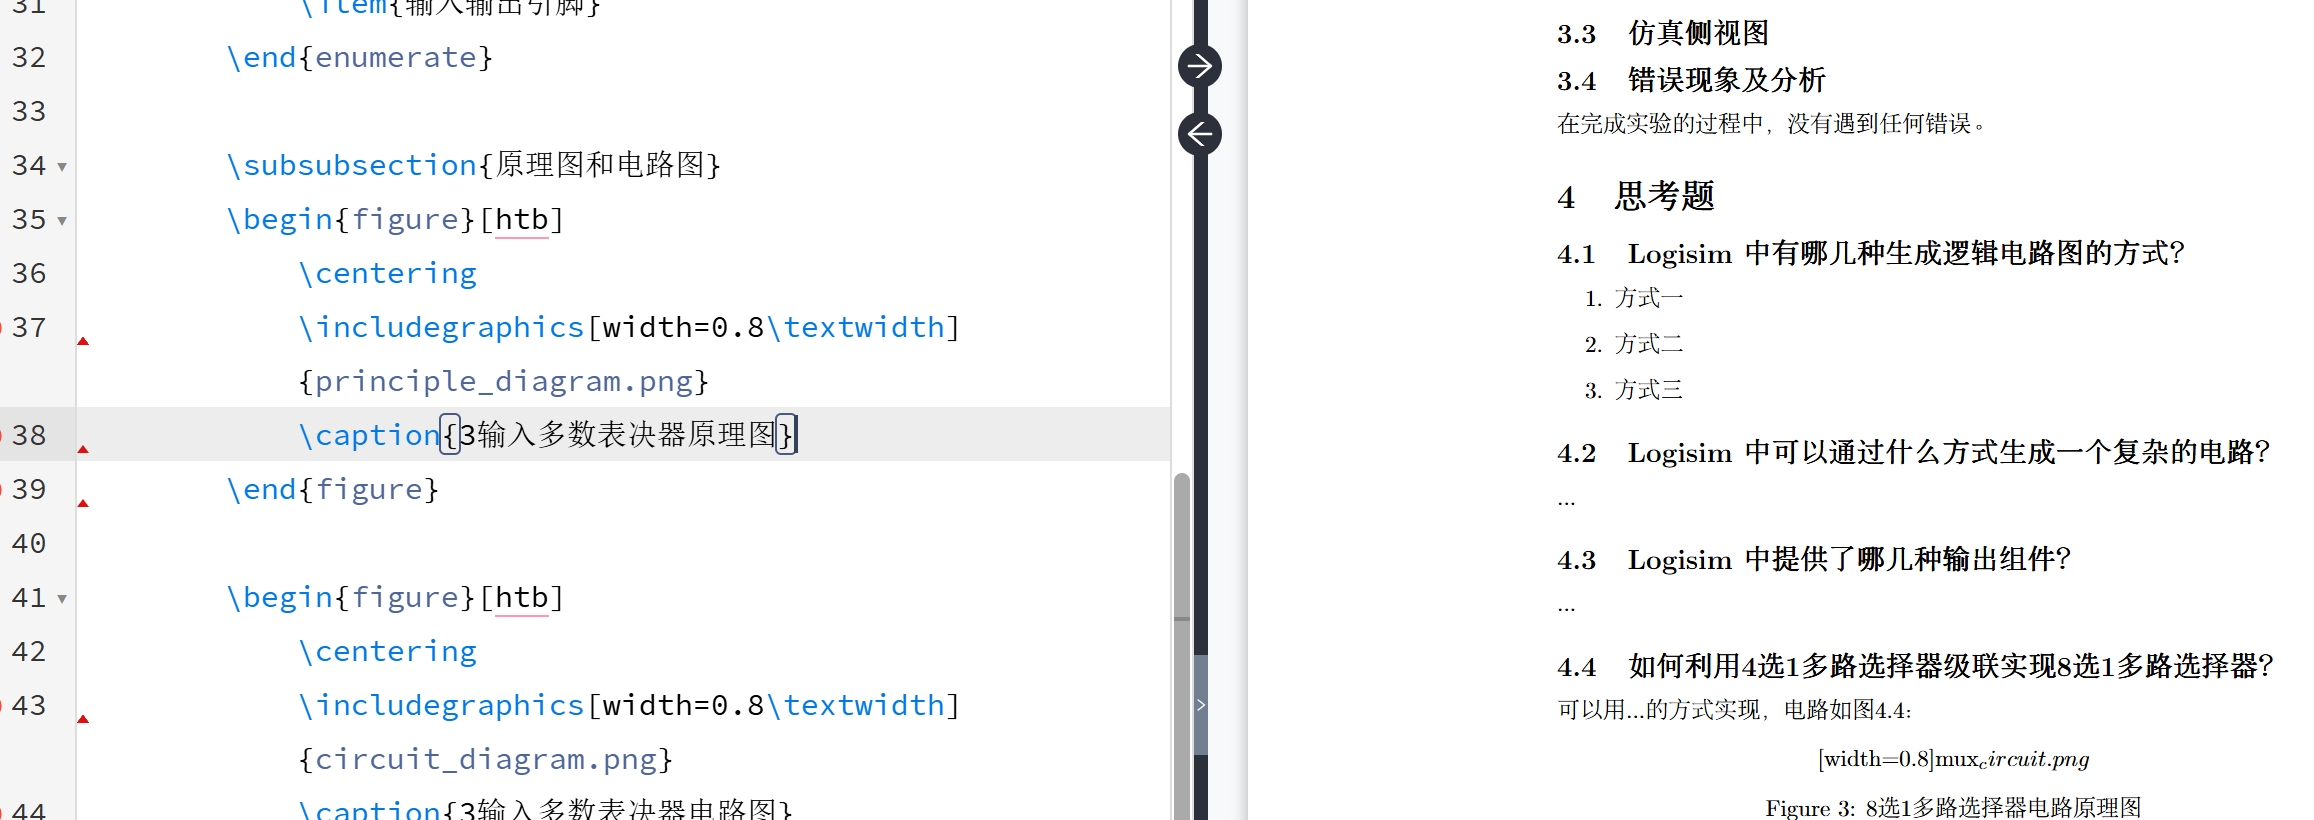
\includegraphics[width=0.8\textwidth]{image.png} % 替换为实际图片文件
  \caption{8选1多路选择器电路原理图}
  \label{8-1MUX}
\end{figure}

\end{document}